\documentclass[a4paper,12pt]{article}

% Input Encoding
\usepackage[utf8]{inputenc}
% Margin Controls
\usepackage[a4paper,bottom=3cm,left=2cm,right=2cm,top=2cm]{geometry}
% Hyphenation libraries
\usepackage[british]{babel}
\usepackage{hardwrap}

% Layout and graphics libraries
\usepackage{graphicx}
\usepackage{wrapfig}
\usepackage{multicol}
\usepackage{tabularx}
\usepackage{url}
\usepackage[perpage,symbol*,bottom,hang,multiple]{footmisc}
\usepackage{tikz}
\usepackage{pdflscape}
\usepackage{etoolbox}
\usetikzlibrary{patterns}

% Page style
\pagestyle{plain}
\newcommand{\fixparskip}{\setlength{\parskip}{4mm plus1mm minus1mm}}
\fixparskip
\setlength{\parindent}{0pt}
\setlength{\columnsep}{1cm}
\renewcommand{\arraystretch}{2}

% Article Environment
\newcommand{\articleAuthor}{}
\newenvironment{article}[2]{
	\pagebreak[2]
	\renewcommand{\articleAuthor}{#2}
	
	{\Huge#1}

	}{

	\notblank{\articleAuthor}{\hfill\Large\articleAuthor}{}
	\vspace{12mm}
	}

\begin{document}
% Title Page
\begin{center}
~ % Non-breaking space so that the page starts, and \vfill evaluates
\vfill

\includegraphics[width=\textwidth,height=0.7\textheight,keepaspectratio]{pictures/cover}
\vfill

\resizebox{!}{16mm}{Picocon 33}

\resizebox{!}{10mm}{Origins}\\
\vspace{1mm}
\resizebox{!}{6mm}{\it{In Medias Res}}

\vspace{5mm}
\resizebox{!}{8mm}{Wyrmtongue}

\thispagestyle{empty}
\end{center}
\clearpage
% End of title page


\begin{article}{The King's Speech}{Anurag Deshpande - ICSF Chair}
	Greetings all, and welcome to the 35th Annual Picocon!

My team of minions have organised a fantastic event for you all, with talks by some awesome guests, some smashing of the dodgiest merch around (although anyone seen harming adorable little porgs will have to face my wrath), and a chance to appreciate some of the worst works of the genre for charity. There's also definitely not a fish duel, and we're actually definitely not erecting a statue in Anurag's honour. 

It has been a great year for the society so far, with many fun and new events, such as the introduction of Themed Fridays and a recent collab with AstroSoc. We encountered a few technical difficulties with converting the library into Atlantis (books + water = bad), which provoked a super sing-a-long ICSF Tour round the various Union Meeting Rooms. We even have T-Shirts to prove it! Apologies if the library isn't in its usual pristine condition - debates over the most efficient sorting algorithm for reshelving the books have yet to be solved. We have plenty of fun events planned for the rest of the term, which are detailed somewhere in this Wyrm. I hope to see you there!

So now it just remains for me to wish you a merry Picocon and a happy smashing things dipped in liquid nitrogen!
\end{article}

\begin{article}{The Sofa's Ramblings}{Noor Mulheron - Picocon Sofa}
	
Hi! My name is Noor, this year's Picocon Sofa (more comfortable than a Chair). Having organised events for the society last year as Chair of Vice, I counted myself just about inexperienced enough to attempt a Picocon, and people seemed to think that trusting me with it would be a good plan! I sincerely hope that over the course of the day this decision proves to be at least not totally ridiculous.

When considering the possibe themes of this year's Picocon, I found myself also thinking of the mythos surrounding how the event began. And so this brought me on to the theme of Origins, where I made a pact with myself to attempt to run Picocon 33 while tracing the beginnings; Picocon 1. My investigations are detailed later in Wyrmtongue!

Of course, I also felt that Picocon 33 would not be complete without a pretentious Latin tagline - and so I tried to combine a comon Latin phrase and a pun of sorts to encompass the second aim I had for Picocon 33. Where my first aim was to trace the origins of Picocon, my second aim was to investigate and discuss how storytelling differs across various forms of media. To combine these ideas, `in medias res', meaning in the middle of things, represents how we are currently in Picocon present, have investigated Picocon past, and Picocon future is optimistic (I hope!). Just as the idea of the past, present and future interlink through the annual event of Picocon, in a similar way, various forms of media interlink by their fundamental aim; to tell a story.

With the theme and tagline neatly decided, I moved on to securing Guests of Honour (GoH's) and the myriad of other tasks assigned to my post. With Paul Cornell's experience in different forms of media, Mihelle Paver's Chronicles of Ancient Darkness series set in the Stone Age origins of humanity, and Carrie Hope Fletcher hailing from the West End, War of the Worlds Musical and a soon-to-be fantasy author, I was lucky enough to secure GoH's who allow for a perfect combination required to explore this year's theme and tagline. 

As is traditional to my role, Picocon 33 has gradually grown and eclipsed most of the things in my life, save perhaps the feeling of excitement and mild terror as the day (today!) approaches. However, despite the obvious additional workload, I have thoroughly enjoyed the process of organising this event - from the beginning to the end.

I hope you all have a wonderful time, and I would like to thank everyone for giving me the chance to run Picocon 33.
\end{article}

\begin{article}{A Word from the Beanbag}{Ben Windo - Picocon Beanbag}
	It is a truth universally acknowledged that a single Picocon in possession of an excellent collection of honourable guests must be in want of attendees, and thus it is to you that we turn, dear reader. I am your Beanbag, provisional second in command. Welcome to the floor show.

The theme for this year’s Picocon is Origins. Picocon is of course cause for celebration, but it is also time for contemplation as we ponder both where we have come from and where we are going. A thought exercise: where were you at this point last year? Hopefully the answer was Picocon, to within a few weeks. Where will you be at this point next year? Hopefully also Picocon.

While you may find yourselves in the midst of the action, this event has been a long time in the making. A shout out to the Sofa, who has tirelessly overcome sleep deprivation, bureaucracy, and even (or so I’ve heard) angry squirrel summoners. A shout out to our legion of volunteers, especially those not currently on the ICSF committee. These noble souls have sacrificed their time and sanity without even the prospect of CV padding, and make the world a better place by their presence.

Whether it be from Abydos, Barsoom, or even Croydon, I’d like to extend a warm welcome to you all. Live long and prosper,

\end{article}

\pagebreak
\begin{article}{Origins}{Noor Mulheron}
	The theme of this year’s Picocon event is ‘Origins’, and so it felt fitting to have an article that explores how the convention came to be. There has been much myth surrounding the origins of Picocon, and so I decided to try and trace back just how the convention began. There are two origin stories – one being that it was a gathering of ICSF members to play board-games at another’s house which they decided to simply escalate; the other being that the first ever Picocon was actually an organised ICSF trip to a different convention in Glasgow, whereupon the group decided that we should make a convention like that ourselves! Picocon’s name was reportedly coined by Steven Barnett, when it was observed that it was a very small convention – earning it the prefix ‘pico’! The year of the first Picocon, however, has been traced back to be the academic year of 1982-1983. Picocon 2 was relatively small and unrecorded, but records survive of the third Picocon, Picocon Pi. This was so named as a pun on the fact that Picocon Pi sounds like Pecan Pie! Picocon has come far over the years, from a trip to a different convention entirely (or board games in a flat!) to a well known London Sci-Fi convention. 
\end{article}

\begin{article}{What's On}{}
	For those of you who don't know, there are many fun events to attend at Picocon. As well as talks by all the Guests of Honour, there is an Author’s Panel where the authors can be asked questions by the attendees. Silly Games is an event where we imitate various gameshows, with general hilarity ensuing, and the Tabletop and Gaming societies run activities as well. We also have an event known simply as ‘Harmless Fun’. 

There are charity events in collaboration with RAG, such as Turkey Readings and Viewings, where books or films are read/shown, but they are so bad that people will pay to prevent them from continuing (or to make it keep going!). We also have ‘Destruction of Dodgy Merchandise’ (DoDM), where examples of terribly misguided merchandise are bid on to be saved or dunked in liquid notrogen and smashed by the highest bidder – the proceeds again going to charity. This year, as last year, Stuart Ashens is coming to Imperial from the Youtube domain to chair the auctioning of the merchandise.

In the evening there will be a showing of the film Le Voyage Dans La Lune, which was the first science-fiction film on the screen, and a Pub Quiz, with the teams captained by our illustrious Guests of Honour! 

We have booksellers and various retailers of items from jewellery to professionally illustrated prints by Autun Purser, and our own stand selling Picocon 33 t-shirts with this year’s logo.
\end{article}

\pagebreak
\begin{article}{Tabletop Gaming at Picocon!}{Dobbin Thomas}
	This year the Tabletop Gaming society will be running boardgames and RPGs in Meeting Room 3 of the union (enter the main entrance, take the lift up to the 3rd floor and the door is on your right). Boardgames will run from 14:30 (just after the author’s panel) until late, where we have lots and lots of games available, short and long to match everyone’s tastes.  We have some of our members around to teach games too, so don’t worry if you don’t know any from our collection.
 
We will also have some role playing games running in meeting room 3 from 18:00! No experience required, just bring your imagination. These will start promptly so please arrive at 6pm or as soon as possible afterwards.
 
Tabletop has regular Boardgame, RPG and Magic events each week of term. Check out our facebook group to find out where and when: www.facebook.com/groups/ImperialCollegeBoardGames/


\end{article}
\begin{article}{Gaming}{Luke Morton – Chair, Imperial College Gaming Club}
	Imperial College Gaming Club may not be associated with the Science Fiction society in any official sense, but we’ve shared a reasonable number of members within the past few years and I myself have many a reason to appreciate Sci-Fi, so the natural step from there is to run something at Picocon.

We’ll have our games consoles set up in Meeting Rooms 1 and 2 from 16:00 – 17:00, and again once all other events have ended at 19:00. We’ll be running our most popular games – namely Super Smash Bros. and Just Dance (it’s much more fun than it sounds). Whether you’re a regular member of Gaming, wanting to reignite an old passion, or even if you haven’t touched a video game in years, I can guarantee you’ll have fun. There’s a good reason why video games are one of the leading causes of procrastination in the country.

And if you happen to be a student, and you’re not yet aware of us (read: if I haven’t pestered you to come to Gaming before), you may like to know that the Club meets on a regular basis, on Wednesdays from 2pm in Room 403A in the EEE building.

I hope you all enjoy Picocon, and find discover/confirm your passion for video games when you come and see us.


\end{article}

\pagebreak
\begin{article}{Schedule}{}
	\vspace{2mm} {\Large} \nopagebreak
\raggedright
\begin{center}
\begin{tabularx}{13cm}{c X l}

09:00 & Front Desk/Registration Opens\footnotemark[1] & \\
09:30 & Author's Talk - Paul Cornell\footnotemark[2] & \\
%10:00& \\
10:30 & Author's Talk - Carrie Hope Fletcher\footnotemark[2]\\
%11:00 & \\
11:30 & Author's Talk - Michelle Paver\footnotemark[2]\\
%12:00 & \\
12:15 & Destruction of Dodgy Merchandise \footnotemark[1]&\\
12:30 & Lunch (see Menu)\footnotemark[3] &\\
%13:00 & \\
13:30 & Author's Panel\footnotemark[2] & \\ 
%14:00 & \\
14:30 & Turkey Readings and Silly Games\footnotemark[2], Boardgames begin \footnotemark[4]&\\
%15:00 & \\
%15:30 & \\
16:00 & Gaming \footnotemark[5]\\
%16:30 & \\
17:00 &  Harmless Fun \it(definitely not a fish duel)\footnotemark[1] &\\
17:30 & Film Showing: \it{Le Voyage Dans La Lune}\footnotemark[3] &\\
18:00 & Pub Quiz (with authors leading teams!) \footnotemark[3], RPGs begin \footnotemark[4]& \\
\end{tabularx}
\end{center}

\footnotetext[1]{Beit Quad}
\footnotetext[2]{Blackett LT1}
\footnotetext[3]{568 and Metric}
\footnotetext[4]{Tabletop gaming events in Meeting Room 3. These will run until late.}
\footnotetext[5]{Meeting Rooms 1 and 2}

\end{article}

\vspace{- 2 cm}

\begin{article}{Lunch Menu}{}
	Food will be served between 12:30-13:30 in Metric, from a mobile servery. Food tickets can be purchased in FiveSixEight and redeemed at the Metric servery. Prices below:

Beef Burger and Chips -£4.75\\
Chicken Burger and Chips - £4.80\\
Veggie Burger and Chips - £4.25\\
Mediterranean roasted vegetable and tomato pasta - £3.95\\
Please note, anyone purchasing any other items from the menu will need to wait as normal as these will be prepared in the main kitchen.
\end{article}

\begin{article}{Guests of Honour}{}

	\begin{tabular}{p{\dimexpr\columnwidth}}
	\\
		{\Large Michelle Paver}

\begin{wrapfigure}{r}{4cm}
	\vspace{-10mm}
	\resizebox{4cm}{!}{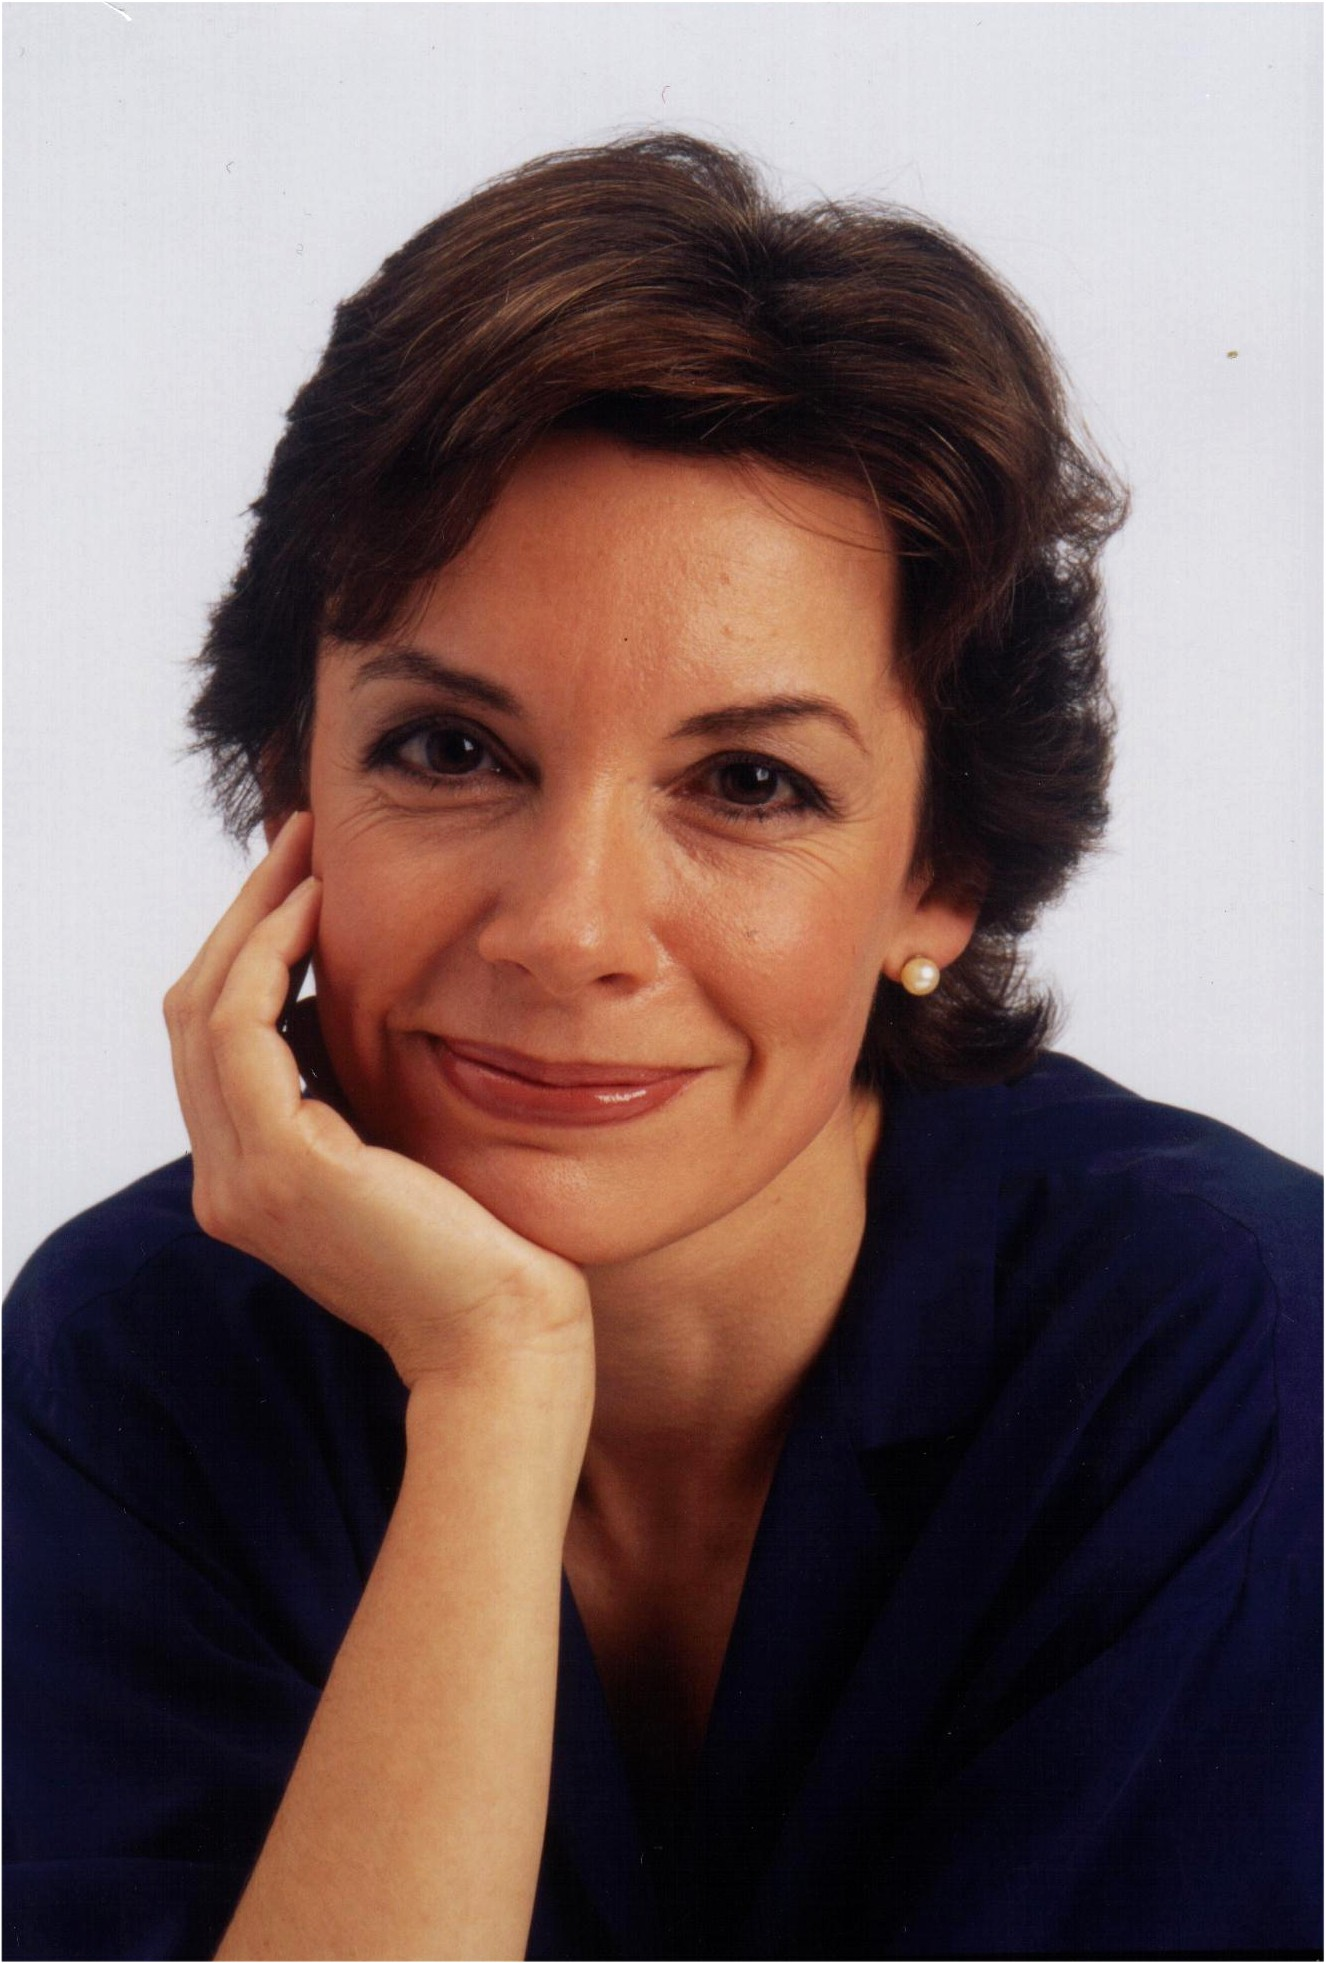
\includegraphics{pictures/michelle}}
	\vspace{-10mm}
\end{wrapfigure}

Author of ‘The Chronicles of Ancient Darkness’, ‘Dark Matter’ and more, she has a first class degree in Biochemistry, and uses her scientific experience in her writing, as well as often going out of her way to experience the things character in her novels go through – even sledding in the Arctic and meeting with wolves!

		\vspace{4cm} ~
	\\
		{\Large Paul Cornell}

\begin{wrapfigure}{r}{4cm}
	\vspace{-10mm}
	\resizebox{4cm}{!}{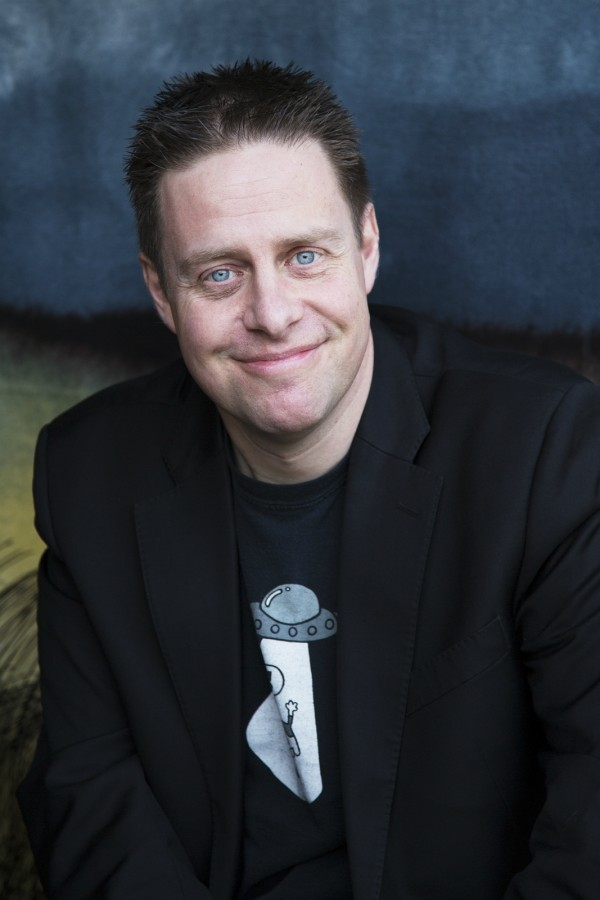
\includegraphics{pictures/paul}}
	\vspace{-10mm}
\end{wrapfigure}

Previous screen-writer for Doctor Who, he has also written several comics and is now an author of the ‘Shadow Police’ series and standalone novels. His experience in many different types of media is unparalleled. 

		\vspace{4cm} ~
	\\
		{\Large Carrie Hope Fletcher}

\begin{wrapfigure}{r}{4cm}
	\vspace{-10mm}
	\resizebox{4cm}{!}{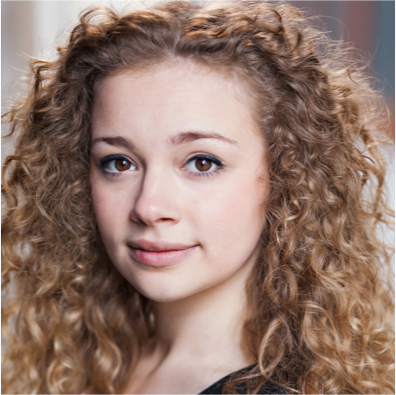
\includegraphics{pictures/carrie}}
	\vspace{-10mm}
\end{wrapfigure}

Having played Beth in the War of the Worlds musical, Carrie Fletcher has experience in storytelling on stage that is being transferred into author-ship. Her debut fantasy novel, ‘On the Other Side’, is coming out this summer, and she has shared snippets of this novel with her large Youtube following. She is currently playing Eponine in the West End in Les Miserables.
	\end{tabular}
\end{article}

\begin{article}{Quest Objectives}{}
	On your way in, you should have been assigned to one of three teams - the Omnics, the Collective, or the Jesters - and given a sticky badge to wear with newfound pride.
If somehow you slipped through the net,
or misplaced your badge,
then go and \emph{politely} berate the receptionists until they give you one.

You will find a list of dangerous, potentially impossible items below.
Find any of these items, bring the evidence back to the front desk, and win fabulous prizes... in the form of points for your team.
Whichever team ends up with the most points will be declared the finest, the greatest, and most importantly the winners!

Now go \emph{for great justice}.

This year's teams are:

\begin{tabular}{ccc}
	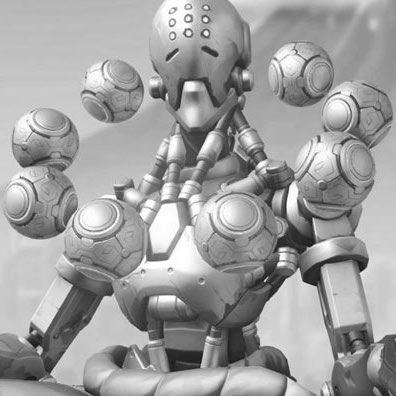
\includegraphics[width=0.2\columnwidth]{pictures/zenyatta} &
	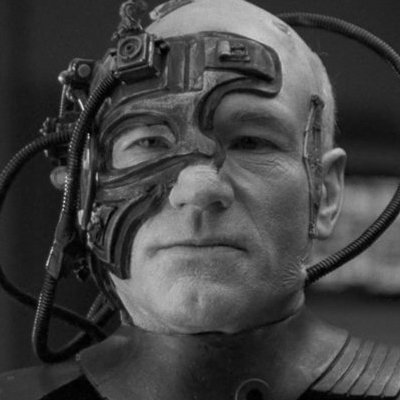
\includegraphics[width=0.2\columnwidth]{pictures/borg} &
	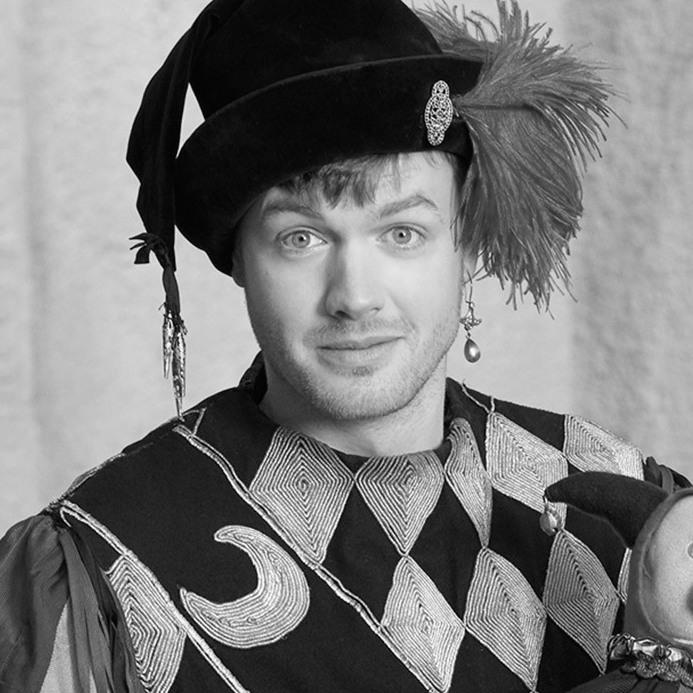
\includegraphics[width=0.2\columnwidth]{pictures/jester} \\

	\parbox{0.3\textwidth}{\center\large The Omnics - be one with the universe} &
	\parbox{0.3\textwidth}{\center\large The Collective - items will be assimilated} &
	\parbox{0.3\textwidth}{\center\large The Jesters - a hunt, but with jazz hands!} \\
\end{tabular}
\vspace{5mm}

These items can be submitted to the Front Desk for Fun Points (after 11am).
Pictures are not (generally) admissible; objective involving people {\textit
must only be undertaken with the other person's permission}.
The front desk reserves the right to keep the submitted items. Each faction may
claim an item on the only once, unless otherwise noted.
\begin{tabbing}
	FD \quad \= Front Desk Person's Discretion\footnotemark \\
	E \> This item may be claimed multiple times per faction (``each'') \\
	M \> For each faction, the highest of their scores will be used
\end{tabbing}
\footnotetext{This actually
	applies to everything; where it is noted, it indicates that you’re
	unlikely to change anyone's mind with your cunning arguments.}

\begin{multicols}{2}
	\begin{tabbing}
1 \hspace{12mm}	\= Little Green Pygmy Solders (E) \\
1	\> Hugs (per person) \\
30	\> Picocon \\
20	\> A non-ICSF fresher at Picocon \\
Age +5	\> Ex-ICSF Chair (M) \\
Age +5	\> Ex-ICSF Librarian (M) \\
Age +5	\> T-shirts from Picocons past (M) \\
10 	\> Previous Guest of Honour (E) \\
10	\> Half of one (1) Dave \\
5	\> The blood of a Picocon first-timer \\
20	\> The Mabbott set \\
8	\> A phylactery \\
80 	\> Dave Clements' phylactery \\
100	\> The Picocon Sofa, calm \\
50	\> The Picocon Beanbag, frantic \\
15	\> Tea, earl grey, hot \\
25 	\> A good drink (FD, E) \\
10 	\> A less good drink (FD) \\
-5	\> Unsatisfactory drink (FD) \\
5	\> Delicious blood (FD) \\
15	\> Spirits from beyond \\
1000 	\> £100 (E) \\
7	\> The contents of my pocketses \\
5	\> Good news (FD, E) \\
-5	\> Bad news (FD, E) \\
1	\> A funny joke (FD, E) \\
-1	\> A bad pun (FD, E) \\
10	\> A charge of EIE/EEE students \\
25	\> A competent barbershop \\ \> quartet (FD) \\
5	\> Any song sung in the style of \\ \> William Shatner \\
50	\> A barbershop quartet in the style \\ \> of William Shatner \\
50 \> Any door to London Below \\
3   \> Newly acquired merchandise  \\
5   \> A teleological proof of the\\ \> existence of a higher power \\
1   \> The solution to the next item \\ \> on the list (E) \\
-1  \> The solution to the previous \\ \> item on the list (E)\\
10  \> Donations of a themed plastic \\ \> abomination \\
5   \> A demon bear (bonus points if fluffy) \\
5   \> A member of the Family of Blood \\
5   \> A little fall of rain \\
5	\> Origami \\
20  \> Dinosaur origami \\
8	\> A Non-Euclidean triangle \\
5   \> A snake eating its own snake tail, \\ \> or snail.\\
5	\> Tribble \\
60	\> Tribble (functional) \\
5	\> A nanosecond \\
10  \> An accretion disk \\
30  \> A terrifying technological terror \\
3	\> A good hat \\
5	\> A correctly fitted top hat \\
5   \> Convincing closet cosplay \\
10  \> Convincing actual cosplay \\
10  \> Pretty trinkets (FD) \\
3   \> The start of something beautiful \\
30   \> The phone from a castle \\
20  \> The phone from a police box \\
50	\> Happiness, $\ge$ 0.1M concentration \\
n(n-1)	\> n Interlocking cogs (functional \\ \> after being poked) (M) \\
10   \> Out of place kerning \\
20   \> An unaired TV pilot \\
20   \> An untelevised air pilot \\
30 	\> A control crystal (with \\ \> demonstration) \\
40 	\> Three quarters of a planck length \\
20 	\> A demonstration of Xeno's paradox \\
10  \> An aesthetically pleasing key (FD)\\
14 	\> A clowder of one cat \\
5   \> The man they call Jayne (or his hat) \\
-50 \> The source of the mysterious ticking noise \\
400	\> The World Turtle \\
800 \> With orbiting bodies \\
10  \> A surviving member of the Imperial \\ \> Steampunk Society \\
50	\> A book ICSF lacks (and wants) \\
1	\> The light at the end of the tunnel \\
5	\> A crowning moment of awesome \\
17	\> Proof humanity's reach extends \\ \> beyond its imagination \\
70  \> A lost Doctor Who episode \\
3	\> Famous last words (subject to \\ \> checking) \\
-1	\> Anything irrelevent (E) \\
-5  \> Anything irrelephant (E) \\
4	\> An Ed (picked up) \\
3	\> Galaxy \\
2	\> A practical application for \\ \> General Relativity \\
4	\> Transcendent understanding \\
10	\> A point in the complex plane \\
5   \> A working AI (demonstrated) \\
10  \> A working AI (safely demonstrated) \\
1000	\> Time machine (points were awarded \\ \> 16th Feb 6pm, ICSF Library, \\ \> password is ``arpeggio'') \\
25	\> A swordfish \\
35	\> A fishsword \\
10	\> A Swan \\
4	\> Nerf Guns \\
3	\> NERV guns \\
10	\> Lab stuff \\
-50	\> per fatality \\
10	\> The Staff of Ra \\
3	\> Positronic brain \\
3	\> Observable Brownian Motion \\
5	\> A fluffy dragon \\
7	\> A plasma generator \\
5	\> Ion cannon (demonstrated) \\
-20	\> Spontaneous combustion \\ \> whilst dancing (E)\\
5	\> A Henry (E)\\
10	\> A Wild Henry\\
10	\> A completed nonogram\\
15	\> A completed crossword\\
	\end{tabbing}
\end{multicols}

{\large Good Luck!}

You're likely to need it...

\end{article}

\begin{article}{Nonogram}{}
	\begin{center}
		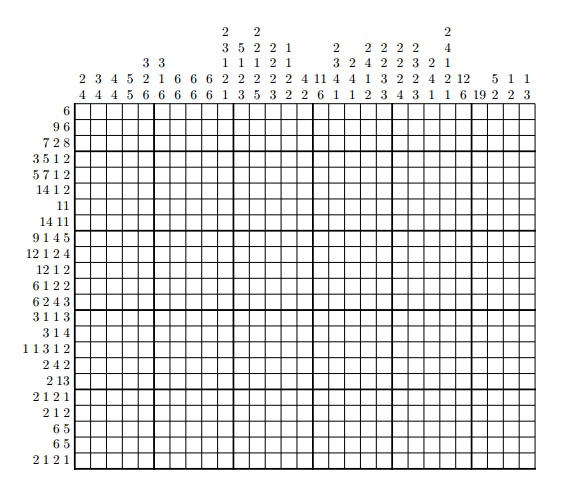
\includegraphics[width=\textwidth,height=0.5\textheight,keepaspectratio]{puzzles/nonogram.jpg}
	\end{center}
\end{article}

\pagebreak

\begin{article}{Crossword}

\begin{center}
	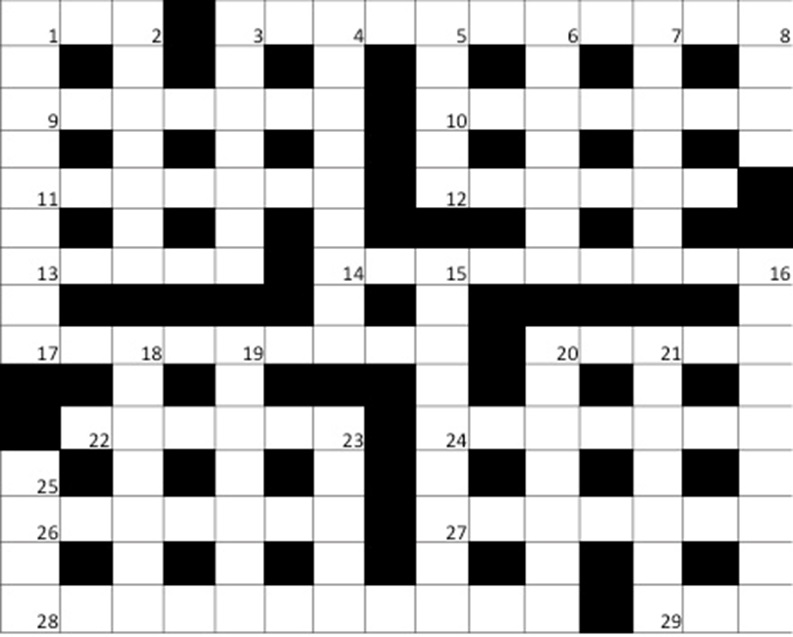
\includegraphics[width=\textwidth,height=0.5\textheight,keepaspectratio]{puzzles/crossword.jpg}
\end{center}

\begin{multicols}{2}
	\input{puzzles/cword.latex}
\end{multicols}

\end{article}

\begin{article}{Map}{}
	\begin{center}
		\resizebox{\columnwidth}{!}{%  Coordinates are shifted and scaled Long/Lat values
%  (0, 0) maps to (-0.1781, 51.5)
%  Rotated clockwise, and slanted into look perpendicular
%  Values have been pre-multipled by 100 to make sure there's no undeflow issues

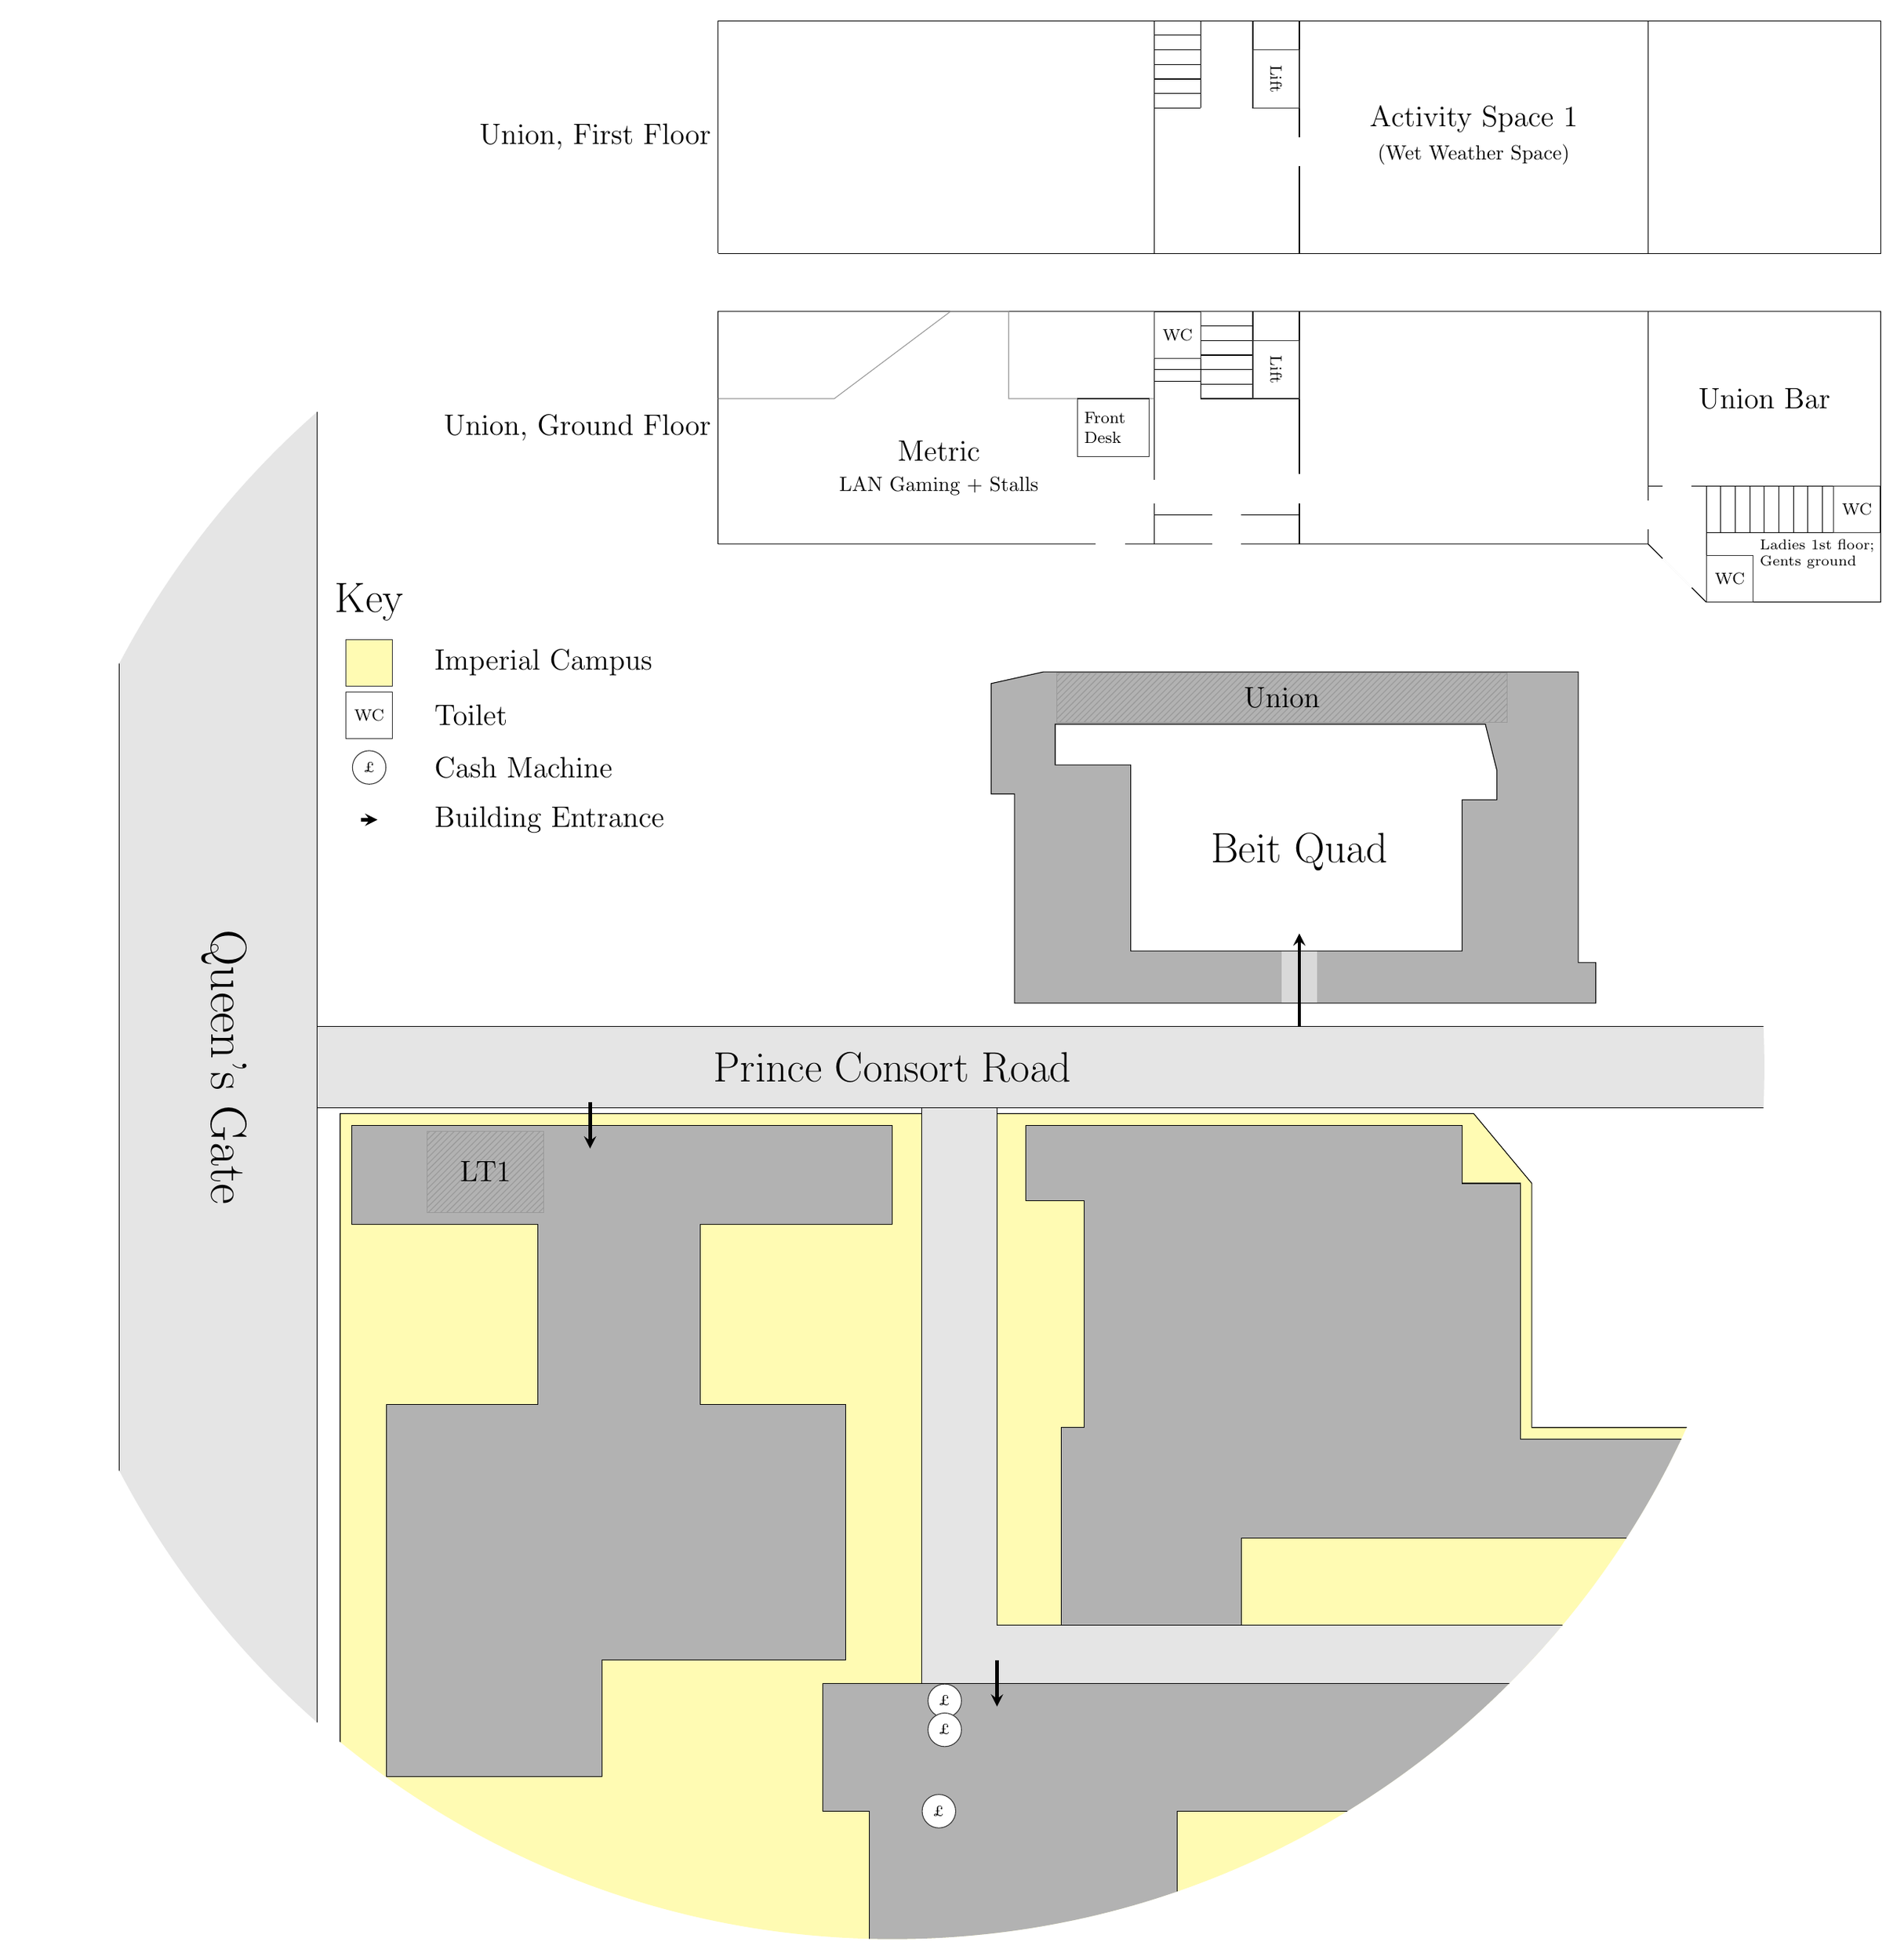
\begin{tikzpicture}

\begin{scope} % Campus Map {{{
\clip (-7,-2) circle (15);

%  Key {{{
\node (key) at (-16, 6) [font=\huge] {Key};
\begin{scope}[font=\Large,minimum height=\baselineskip,minimum width=\baselineskip];

	\node at ([below=6mm] key.south) [minimum width=8mm,minimum height=8mm,fill=yellow!30,draw=black!80] {};
	\node at ([below=6mm, right=10mm] key.south) [right] {Imperial Campus};

	\node at ([below=15mm] key.south) [minimum width=8mm,minimum height=8mm,fill=white,draw=black!80,font=\footnotesize] {WC};
	\node at ([below=15mm, right=10mm] key.south) [right] {Toilet};

	\node at ([below=24mm] key.south) [circle,fill=white,draw=black!80,font=\scriptsize] {\textsterling};
	\node at ([below=24mm, right=10mm] key.south) [right] {Cash Machine};

	\coordinate (entkey) at ([below=33mm] key.south);
	\draw [->,>=stealth,ultra thick] ([left=4pt] entkey) -- ([right=4pt] entkey);
	\node at ([below=33mm, right=10mm] key.south) [right] {Building Entrance};
\end{scope}
%}}}

% Beit Quad (Outer) {{{
\draw[fill=gray!60]
		(  5.1, - 0.9) --
		(  5.1, - 0.2) --
		(  4.8, - 0.2) --
		(  4.8,   4.8) --
		(- 4.4,   4.8) --
		(- 5.3,   4.6) --
		(- 5.3,   2.7) --
		(- 4.9,   2.7) --
		(- 4.9, - 0.9) --
		cycle
	; %}}}

% Beit Quad (Archway) {{{
\draw[fill=gray!30,draw=gray!30]
		(- 0.3, - 0.88) --
		(- 0.3,   0.01) --
		(  0.3,   0.01) --
		(  0.3, - 0.88) --
		cycle
	; %}}}

% Beit Quad (Inner) {{{
\draw[fill=white]
		(  2.8,   2.6) --
		(  3.4,   2.6) --
		(  3.4,   3.1) --
		(  3.2,   3.9) --
		(- 4.2,   3.9) --
		(- 4.2,   3.2) --
		(- 2.9,   3.2) --
		(- 2.9,   0.0) --
		(  2.8,   0.0) --
		cycle
	; %}}}

\node at ( 0,  1.7) [font=\huge] {Beit Quad};

\node[minimum width=7.75cm,minimum height=0.85cm,font=\Large,
	pattern=north east lines,pattern color=black!40,draw=black!40]
	at (-0.3,4.36) {Union};

%  Imperial Campus {{{
\draw[fill=yellow!30]
		(-16.5, - 2.8) --
		(  3.0, - 2.8) --
		(  4.0, - 4.0) --
		(  4.0, - 8.2) --
		( 10.0, - 8.2) --
		( 10.0, - 2.8) --
		( 20.0, - 2.8) --
		( 20.0, -21.0) --
		(-16.5, -21.0) --
		cycle
	; %}}}

% Blackett / Huley {{{
\draw[fill=gray!60]
		(-16.3, - 3.0) --
		(-16.3, - 4.7) --
		(-13.1, - 4.7) --
		(-13.1, - 7.8) --
		(-15.7, - 7.8) --
		(-15.7, -14.2) --
		(-12.0, -14.2) --
		(-12.0, -12.2) --
		(- 7.8, -12.2) --
		(- 7.8, - 7.8) --
		(-10.3, - 7.8) --
		(-10.3, - 4.7) --
		(- 7.0, - 4.7) --
		(- 7.0, - 3.0) --
		cycle
	; %}}}

\node [minimum height=1.4cm,minimum width=2cm,pattern=north east lines,
	pattern color=black!40,draw=black!40,font=\Large]
	at (-14, -3.8) {LT1};

% That Random Building (Group) {{{
\draw[fill=gray!60]
		(- 4.7, - 4.3) --
		(- 3.7, - 4.3) --
		(- 3.7, - 8.2) --
		(- 4.1, - 8.2) --
		(- 4.1, -11.6) --
		(- 1.0, -11.6) --
		(- 1.0, -10.1) --
		( 10.0, -10.1) --
		( 10.0, - 8.4) --
		(  3.8, - 8.4) --
		(  3.8, - 4.0) --
		(  2.8, - 4.0) --
		(  2.8, - 3.0) --
		(- 4.7, - 3.0) --
		cycle
	; %}}}

% Sherfield / Library {{{
\draw[fill=gray!60]
		( 13.4, -12.6) --
		(- 8.2, -12.6) --
		(- 8.2, -14.8) --
		(- 7.4, -14.8) --
		(- 7.4, -17.2) --
		(- 8.0, -17.2) --
		(- 8.0, -20.3) --
		(- 1.1, -20.3) --
		(- 1.1, -17.2) --
		(- 2.1, -17.2) --
		(- 2.1, -14.8) --
		( 13.4, -14.8) --
		cycle
	; %}}}

% Calendar Road {{{
\draw[fill=gray!20]
		(- 6.5, -12.6) --
		(  5.2, -12.6) --
		(  5.2, -11.6) --
		(- 5.2, -11.6) --
		(- 5.2, - 2.7) --
		(- 6.5, - 2.7) --
		cycle
	; %}}}

% Prince Consort Road {{{
\draw[fill=gray!20]
		( 23.3, - 1.3) --
		(-17.5, - 1.3) --
		(-17.5, - 2.7) --
		( 23.3, - 2.7) --
		cycle
	; %}}}

\node at (-7, -2) [font=\huge] {Prince Consort Road};

% Queen's Gate {{{
\draw[fill=gray!20]
		(-16.9, -18.7) --
		(-16.9, 15.3) --
		(-20.3, 15.3) --
		(-20.3, -18.7) --
		cycle
	; %}}}

\node at (-18.5, -2) [rotate=-90,font=\Huge] {Queen's Gate};

% Useful Entrances
\draw[->,>=stealth,ultra thick] (0, - 1.3) -- (0,  0.3); % Beit
\draw[<-,>=stealth,ultra thick] (-5.2,-13.0) -- (-5.2,-12.2); % Sherfield
\draw[<-,>=stealth,ultra thick] (-12.2,-3.4) -- (-12.2,-2.6); % Blackett

\end{scope} %}}}

\begin{scope}[shift={(-10,7)}] % Union Floor G Map {{{

	\draw (0, 0) -- (16, 0) -- (17, -1) -- (20, -1) -- (20, 4) -- (0, 4) -- (0,0) node [pos=0.5,left,font=\Large] {Union, Ground Floor};

	\draw (7.5, 0.5) -- (10, 0.5); % Inner Doors
	\draw (7.5,  0) -- (7.5,  4); % Metric / Hall
	\draw (10, 0) -- (10, 4); % Hall / 568
	\draw (16, 0) -- (16, 4); % 568 / Union Bar
	\draw (16, 1) -- (20, 1); % South of Union Bar
	\draw (17,-1) -- (17, 1); % East of NE corner entrance

	% NE steps to ladies
	\foreach \x in {17.25,17.5,17.75,18,18.25,18.5,18.75,19}{
		\draw (\x, 1) -- (\x, 0.2);
	}
	\draw (17, 0.2) -- (19.25, 0.2);

	% Main staircase
	\foreach \y in {2.5, 2.75, 3, 3.25, 3.5, 3.75}{
		\draw (8.3,\y) -- (9.2,\y);
	}
	\draw (8.3, 2.5) -- (8.3, 4);
	\draw (9.2, 2.5) -- (9.2, 4);

	% Stairs down to 'ground floor' toilets
	\foreach \y in {2.8, 3, 3.2}{
		\draw (7.5,\y) -- (8.3,\y);
	}

	% Main lift
	\node at (9.6, 3) [rotate=-90,font=\footnotesize,minimum height=8mm,minimum width=10mm,draw=black!80] {Lift};

	% Toilets
	\node at (7.5,4) % Main entry, both (steps! :/)
		[below right,minimum width=8mm,minimum height=8mm,fill=white,draw=black!80,font=\footnotesize] {WC};
	\node at (20,1) % NE, Ladies (1st Floor)
		[below left,minimum width=8mm,minimum height=8mm,fill=white,draw=black!80,font=\footnotesize] {WC};
	\node at (17,-1) % NE, Gents (outside Union Bar)
		[above right,minimum width=8mm,minimum height=8mm,fill=white,draw=black!80,font=\footnotesize] {WC};
	\node at (17.8,0.2) [below right,text width=2cm,font=\scriptsize] {Ladies 1st floor;\\ Gents ground};

	% Doors
	\begin{scope}[draw=white!100,thick]
		\draw (8.5,0) -- (9,0); % Main entrance
		\draw (8.5,0.5) -- (9,0.5); % Main entrance inner

		\draw (6.5,0) -- (7,0); % Metric external
		\draw (7.5,0.7) -- (7.5,1.1); % Metric internal

		\draw (10,0.7) -- (10,1.2); % 568 Internal

		\draw (16,0.25) -- (16,0.75); %568 <-> NE
		\draw (16.25,-0.25) -- (16.75,-0.75); % NE External
		\draw (16.25,1) -- (16.75,1); % Union bar
	\end{scope}

	% Rooms
	\node at (18,2.5) [font=\Large] {Union Bar};
	\node (met) at (3.8,1.6) [font=\Large] {Metric};
	\node at ([below=0.6cm] met) {LAN Gaming + Stalls};

	% Metric detailing
	\draw [draw=black!40] (7.5,2.5) -- (5,2.5) -- (5, 4) -- (4,4) -- (2,2.5) -- (0,2.5);
	\node at (6.8,2) [draw=black!80,text width=1cm,minimum width=1cm,minimum height=1cm,font=\footnotesize] {Front Desk};
\end{scope} %}}}

\begin{scope}[shift={(-10,12)}] % Union Floor 1 Map {{{

	\draw (0, 0) -- (20, 0) -- (20, 4) -- (0, 4) -- (0,0) node [pos=0.5,left,font=\Large] {Union, First Floor};

	\draw (7.5,  0) -- (7.5,  4); % Metric / Hall
	\draw (10, 0) -- (10, 4); % Hall / 568
	\draw (16, 0) -- (16, 4); % 568 / Union Bar

	\foreach \y in {2.5, 2.75, 3, 3.25, 3.5, 3.75}{
		\draw (7.5,\y) -- (8.3,\y);
	}
	\draw (8.3, 2.5) -- (8.3, 4);
	\draw (9.2, 2.5) -- (9.2, 4);
	\node at (9.6, 3) [rotate=-90,font=\footnotesize,minimum height=8mm,minimum width=10mm,draw=black!80] {Lift};

	% Doors
	\begin{scope}[draw=white!100,thick]
		\draw (10, 1.5) -- (10, 2);
	\end{scope}

	\node (as1) at (13, 2.3) [font=\Large] {Activity Space 1};
	\node at ([below=0.6cm] as1) {(Wet Weather Space)};
\end{scope} %}}}

% Cash Points {{{
\node at (- 6.1,-12.9) [circle,fill=white,draw=black!80,font=\scriptsize] {\textsterling};
\node at (- 6.1,-13.4) [circle,fill=white,draw=black!80,font=\scriptsize] {\textsterling};
\node at (- 6.2,-14.8) [circle,fill=white,draw=black!80,font=\scriptsize] {\textsterling};
%}}}

\end{tikzpicture}

}
	\end{center}
\end{article}

\end{document}
